\documentclass{standalone}
\usepackage{ tikz }
\usetikzlibrary{shapes}
\usetikzlibrary{plotmarks}
\usepackage{ xparse }

\usepackage{../../../macros}
\usetikzlibrary{calc}

\begin{document}
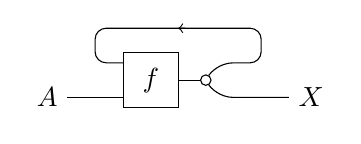
\begin{tikzpicture}[yscale=-1,x=1em,y=1.25em]

    \node [anchor=east] at (-1,0) {$A$};
    \draw (-1,0) -- (1,0);
    \node[draw, minimum height = 2em, minimum width = 2em, anchor = west, fill=white] at (1,-0.5){$f$};
    \draw (3,-0.5) -- (4,-0.5); 
    \node (C1) [draw, circle, fill=white, scale=0.4] at (4,-0.5) {};
    \coordinate (X1) at (5,0);
    \coordinate (X2) at (7,0);
    \coordinate (T1) at (5,-1);
    \coordinate (AR) at (3,-2);
    \node (X) [anchor=west] at (7,0) {$X$};

    \draw (C1) to [out=285, in=180] (T1);
    \draw (C1) to [out=75, in=180] (X1) to (X);

    \draw [rounded corners, ->] (T1) -- ($(T1) +(1,0)$) -- ($(T1) +(1,-1)$) -- (AR);
    \draw [rounded corners] ($(AR) +(0.25,0)$) -- (0,-2) -- (0,-1) -- (1,-1);

\end{tikzpicture}
\end{document}